\documentclass[a4paper]{article}

% Packages
\usepackage[left=25mm, top=30mm,]{geometry}
\usepackage{graphicx}
\usepackage{float}
\usepackage{siunitx}
\usepackage{listings}
\usepackage{physics}
\usepackage[dutch]{babel}
\usepackage{fixltx2e}
\usepackage{amsmath}
\usepackage{amsfonts}
\usepackage{amssymb}
\usepackage[noend]{algpseudocode}
\usepackage{algorithm}

\renewcommand{\lstlistingname}{Algoritme}
\renewcommand{\lstlistlistingname}{Lijst van algoritmen}
\newcommand*{\qed}{\hfill\ensuremath{\square}}

\makeatletter
\renewcommand{\ALG@name}{Algoritme}
\makeatother

\lstset{
	language=Matlab,
	captionpos=b,
	frame=single,
	numbers=left,
	numberstyle=\tiny\color{{rgb}{0.5,0.5,0.5}},
	showstringspaces=false,
}

\usepackage{hyperref}
\hypersetup{pdfborder={0 0 0}}

% Commands and stuff
\newcommand{\opgave}[1]{\subsection{Opgave #1}}

% Title Page stuff
\title{Practicum Numerieke Modelering en Benadering}
\author{Wim Kunnen, r0629332 \\ Bo Kleynen, r0624034}
\date{7 mei 2018}

% Actual document
\begin{document}

\begin{titlepage}
\maketitle
\thispagestyle{empty}
\end{titlepage}


% Table of Contents
\pagenumbering{roman}
\setcounter{page}{1}
\tableofcontents
\cleardoublepage

% List of figures
\listoffigures
\addcontentsline{toc}{section}{\numberline{} Lijst van figuren}

% List of Tables
\listoftables
\addcontentsline{toc}{section}{\numberline{} Lijst van tabellen}

\listofalgorithms
\addcontentsline{toc}{section}{\numberline{} Lijst van algoritmen}

\cleardoublepage



\pagenumbering{arabic}
\setcounter{page}{1}

% PDE stuff
\section{Theoretische eigenschappen}\label{sec:theorie}

\opgave{1: Gelijktijdige iteratie}\label{sec:oef1}

Gelijktijdige iteratie geeft convergentie naar de grootste eigenwaarde. Door gelijktijdige iteratie toe te passen op de matrix $(A-\tau I)^{-1}$ worden de eigenwaarden $\frac{1}{\lambda - \tau}$ gevonden. Hierin zijn $\lambda$ de originele eigenwaarden en is de grootste eigenwaarde deze die het dichtst gelegen is bij $\tau$. Hiervoor wordt een ander algoritme gebruikt opdat men niet de inverse expliciet zou moeten bepalen, maar men een stelsel kan oplossen.
\newline
\begin{algorithm}
\begin{algorithmic}[H]\label{alg:SI}\caption{Simultaneous iteration with shifts}
	\State $M = (A-\tau I)^{-1}$
	\State Pick $\textbf{\^{Q}}^{(0)} \in  \mathbb{R^{\text{m} \times \text{n}}}$
	\For{$k = 1, 2, ...$}
		\State $\textbf{Z} = \textbf{A}\textbf{\^{Q}}^{(k-1)}$
		\State$\textbf{\^{Q}}^{(k)}\textbf{\^{R}}^{(k)} = \textbf{Z}$
	\EndFor
\end{algorithmic}
\end{algorithm}

\opgave{2: Rayleigh iteratie}\label{sec:oef2}
a) Wanneer $\lambda_{k-1}$ dichter komt bij de exacte eigenwaarde, zal er een een eigenwaarde van de matrix $A-\mu I$ dichter tegen nul liggen. Het stelsel wordt dus (bijna) singulier.  De overeenkomstige eigenwaarde van de ge\"inverteerde matrix $(A-\mu I)^{-1}$ zal heel groot worden, aangezien de eigenwaarden van de inverse van een matrix gelijk zijn aan de inversen van de eigenwaarden van de oorspronkelijke matrix.  We krijgen dus een grote fout op de oplossing in de richting van de overeenkomstige eigenvector. Deze eigenvector is gelijk aan de eigenvector van de overeenkomstige eigenwaarde van de niet ge\"inverteerde matrix.  De gevonden vector ligt dus al in de juiste richting (die van de te zoeken eigenvector bij de eigenwaarde), maar zal door het zeer slechte conditiegetal heel groot zijn. Na normalisatie vinden we echter een vector die de gezochte eigenvector zeer goed benadert.\\
\newline
b) \\  Het zoeken naar een waarde $\rho \in \mathbb{R}$ waarvoor geldt dat:
\begin{equation}
\min_{\rho \in \mathbb{R}} ||Ax - \rho x||_2
\end{equation}
komt overeen met het zoeken van een kleinste-kwadraten benadering van:
\begin{equation}
x \rho \approx Ax
\end{equation}
waarbij $x$ een $m \cross 1$ matrix en $Ax$ het rechterlid is.
De normaalvergelijking is:
\begin{equation}
x^T x \rho = x^T A x
\end{equation}
of anders geschreven:
\begin{equation}
\rho = \frac{x^T A x}{x^T x}
\end{equation}
hetgeen overeenkomt met het Rayleigh quoti\"ent van $x$.

\opgave{3: Methode van Arnoldi}\label{sec:oef3}
a)  \\
\newline
b)  Zij $\vec{v} \in K_n$. Aangezien $Q_n$ een orthogonale basis vormt voor $K_n$, is $\vec{v} = Q_n\vec{x}$ voor een $\vec{x} \in \mathbb{C^{\text{n}}}$. Nu is $A \vec{v} = AQ_n\vec{v} = Q_n(H_n\vec{x}) = Q_n\vec{y}$, met $\vec{y} = H_n\vec{x} $.  Waaruit volgt: $A\vec{v} \in K_n$. \qed\\
\newline
c) De $n+1^e$ basisvector van $K_{n+1}$ wordt gegeven door $ A^nb = A(A^{n-1b}) $. Uit b) volgt: $A^nb \in K_n$. Dus $K_{n+1} \subseteq K_n$ en $K_{n} \subseteq K_{n+1}$ zijn triviaal. Hieruit volgt dat: $K_n = K_{n+1}$ en via inductie, $K_n = K_{n+i}$ voor $1 \leq i \leq (m-n)$\\
\newline
d) Zij $\vec{v}$ een eigenvector van $H_n$ met eigenwaarde $\lambda$. Uit b) weten we $AQ_n = Q_nH_n$. Dus $A(Q_n\vec{v}) = Q_nH_n\vec{v} = \lambda(Q_n\vec{v})$. Waaruit volgt dat elke eigenwaarde van $H_n$ ook een eigenwaarde is van A.\\
\newline
e) $\vec{x} = A^{-1}b = A^{-1}Q_n\vec{e_1}\norm{b} = A^{-1}Q_nH_nH_n^{-1}\vec{e_1}\norm{b} = A^{-1}AQ_nH_n^{-1}\vec{e_1}\norm{b} = Q_n(H_n^{-1}\vec{e_1}\norm{b}) \in K_n$.

\section{Het QR-algoritme}\label{sec:QR}

\opgave{4: Hessenberg}\label{sec:oef4}

De Hessenbergvorm van een matrix is een matrix waarvoor alle elementen onder de eerste benedendiagonaal gelijk zijn aan nul.
\begin{equation}\nonumber
	h_{ij} =0 , \text{voor alle } i > j+1
\end{equation}

We zien inderdaad deze vorm. Ook staan er nullen waar ze niet moeten staan, maar de definitie meldt niets over het niet nul zijn van deze elementen. Veel algoritmen hebben beduidend minder rekenkracht nodig wanneer deze toegepast worden op diagonale matrices. Deze eigenschap komt ook vaak voor wanneer de berekeningen uitgevoerd worden op een Hessenbergmatrix.
\begin{figure}[H]
	\begin{center} 
		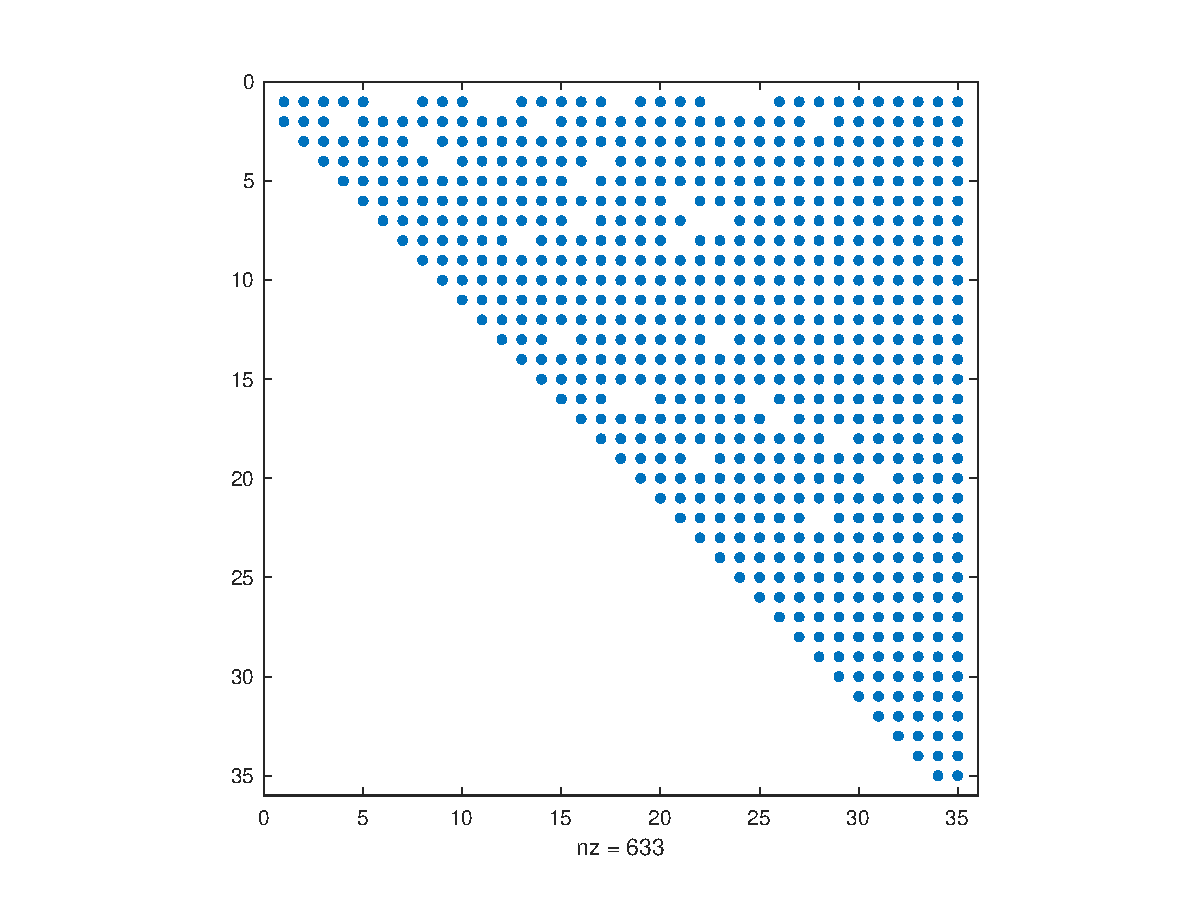
\includegraphics[width=0.5\textwidth]{spy.eps}
	\end{center}
	\caption{Sparsiteit van de gegeven matrix.}
	\label{fig:spy}
\end{figure}
\newpage

\opgave{5: Implementatie QR-algoritmen}\label{sec:oef5}
De algoritmen werden uitgewerkt in bijgevoegde Matlab files en de fout geplot in functie van het aantal iteratie stappen voor de gegeven matrix mat1. Zoals verwacht vertonen de algoritmen kwadratische convergentie, waarbij die met shifts sneller convergeren.

\begin{figure}[H]
	\begin{center} 
		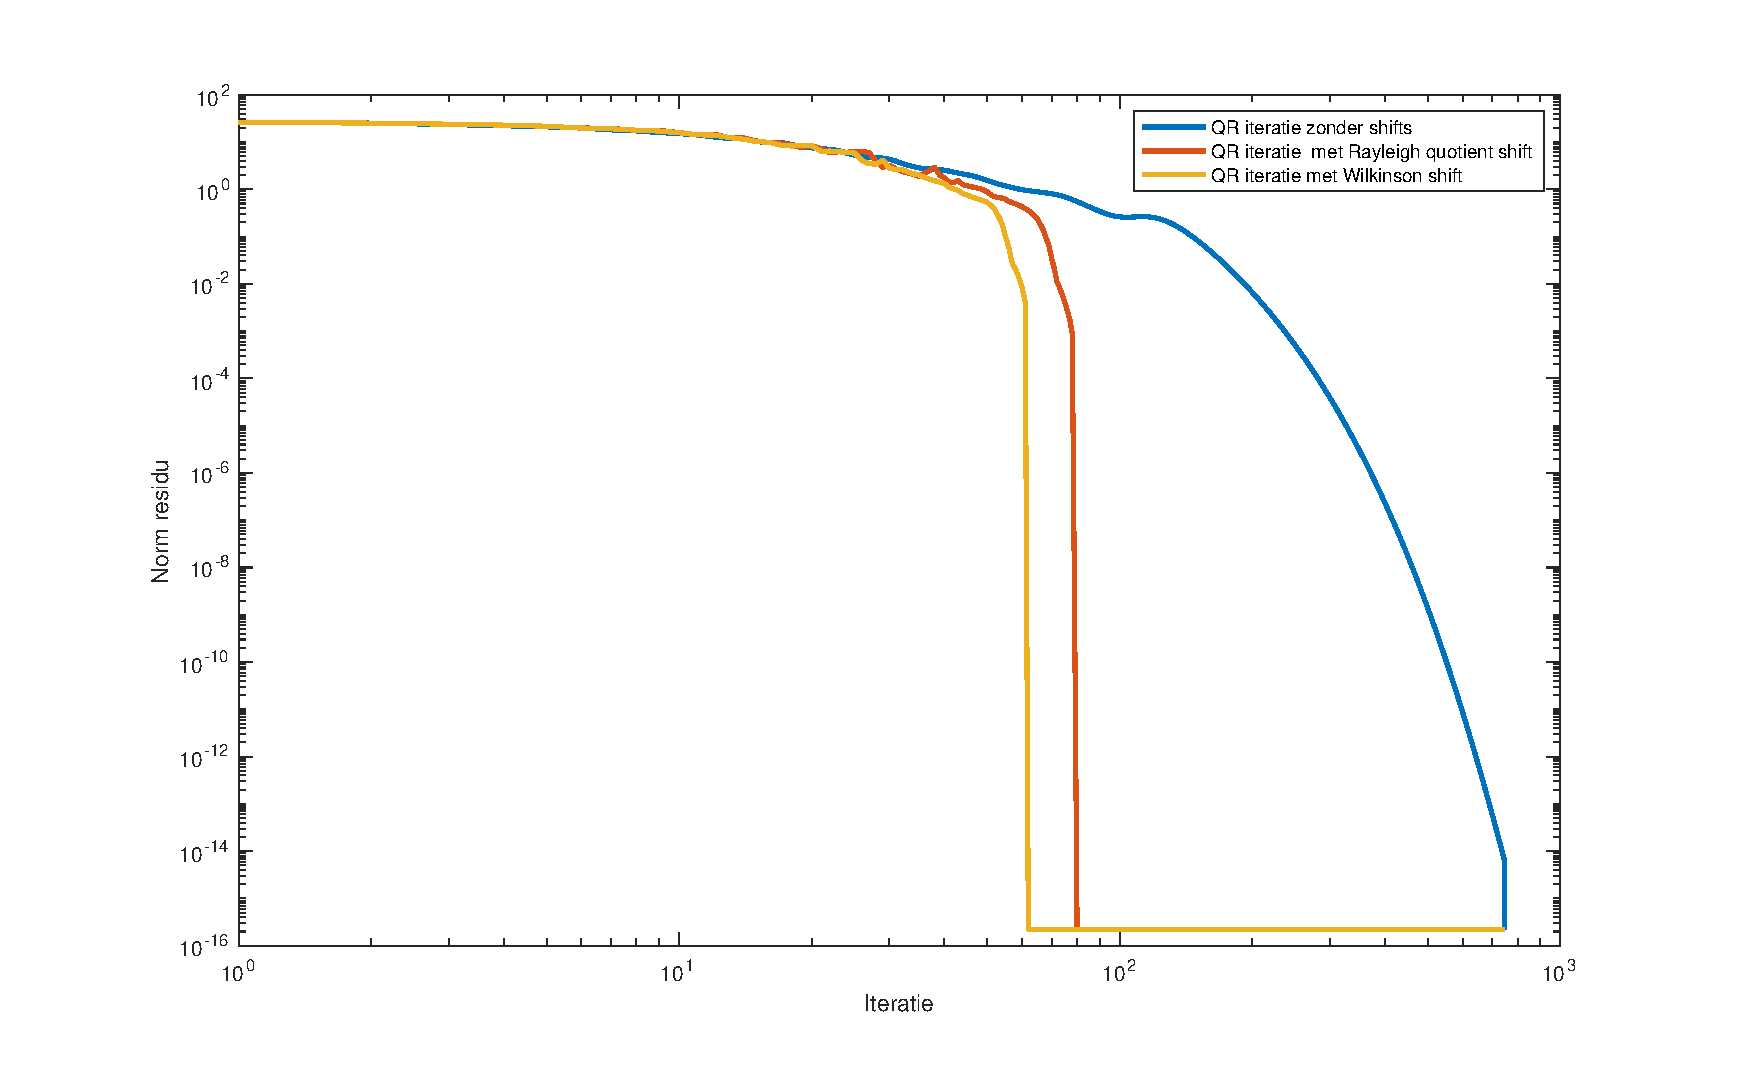
\includegraphics[width=0.7\textwidth]{opgave5.eps}
	\end{center}
	\caption{Convergenties QR algoritmen.}
	\label{fig:QR}
\end{figure}

\opgave{6: Vergelijking}\label{sec:oef6}

De methode van de gelijktijdige iteratie zal alle mogelijke eigenwaarden vinden, terwijl het 	 QR-algoritme en de Rayleigh quoti\"ent iteratie er maar 1 vinden. \par\noindent 
    Het QR-algoritme met Rayleighshift lijkt op de Rayleigh quoti\"ent iteratie, omdat we door 		toepassing van het Rayleigh quoti\"ent dezelfde eigenwaarde en eigenvector benadering krijgen 	  na de shift als bij de Rayleigh quoti\"ent iteratie. Hierdoor heeft het QR-algoritme dus net 		zoals de Rayleigh quoti\"ent iteratie een kwadratische convergentie. \par\noindent
    De gelijkenis tussen het QR algoritme en de gelijktijdige iteratie, is dat het QR-algoritme 	eigenlijk het gelijktijdige iteratie algoritme is, maar dan toegepast op de identiteitsmatrix. 	   Doordat we nu met vierkant matrices werken, kunnen we dan ook het volledige QR-factorisatie 		toepassen.
    \\ \par\noindent
    De convergentie van het QR-algoritme met Rayleighshift is een combinatie van de convergentie 	 van Rayleigh iteratie en gelijktijdige iteratie, in het opzicht dat zowel het QR-algoritme als 	de Rayleigh iteratie kwadratisch convergeren, terwijl gelijktijdige iteratie slechts lineair 	 convergeert. In Figuur 2 is de eerste iteratie al zeer nauwkeurig, waardoor dit niet duidelijk 	zichtbaar is. Het QR-algoritme is net zoals bij gelijktijdige iteratie minder afhankelijk van 	  de initi\"ele startvector. De Rayleigh quoti\"ent iteratie zal convergeren naar de 				dichtstbijzijnde eigenwaarde en eigenvector. Indien er dus geen eigenwaarde in de buurt ligt, 	  zal de convergentie traag verlopen. QR is dus een goede combinatie van de twee, voor het geval 	 er slecht \'e\'en eigenwaarde gekend moet zijn, omdat er altijd convergentie optreedt en deze 		relatief snel verloopt.
\newpage

\section{Alternatieve eigenwaardenalgoritmen}\label{sec:alternatief}

\opgave{7: Co\"effici\"enten}\label{sec:oef7}

Een rotatie-matrix is een orthogonale matrix met: 
\begin{equation} \label{eq:rot-matrix}
det(J)=1
\end{equation}.
We zoeken een oplossing voor: 
\begin{equation} \label{eq:jacobi}
J^T 
\begin{bmatrix} a & d \\ d & b \end{bmatrix} 
J = 
\begin{bmatrix}\ne{0} & 0 \\ 0 & \ne{0}\end{bmatrix}
\end{equation}

met: $$J = \begin{bmatrix}
c & s \\ -s & c
\end{bmatrix}$$

Uitwerken van \ref{eq:jacobi} levert volgende vergelijking op:
\begin{equation}
c^2d-bcs+acs-ds^2 = 0
\end{equation}

Samen met \ref{eq:rot-matrix} vormt dit een stelsel van 2 vergelijkingen met 2 onbekenden.
$$\begin{cases}
c^2d-bcs+acs-ds^2 = 0 \\ det(J) = c^2 + s^2 = 1
\end{cases}$$

We voeren volgende substitutie uit op \ref{eq:jacobi}
\begin{equation}
\begin{cases}
c = cos(\theta) \\ s = sin(\theta)
\end{cases}
\end{equation}

$$ d \cos^2(\theta) - b \cos(\theta) \sin(\theta) + a \cos(\theta) \sin(\theta) - d \sin^2(\theta) = 0$$
$$ d \cos(2\theta) + \frac{a-b}{2}(2 \cos(\theta)\sin(\theta)) = 0 $$
$$ d \cos(2\theta) = \frac{b-a}{2}\sin(2\theta)$$

\begin{equation}
tan(2\theta) = \frac{2d}{b-a}
\end{equation}

\opgave{8: Implementatie Jacobi}\label{sec:oef8}

\begin{algorithm}
\begin{algorithmic}[H]\label{alg:SI}\caption{Jacobi}
\State $m = size(rows(D))$
\While{$\norm{R_A}_F > tol$}
\For{$i = 1:m-1$}
\For{$j = i+1:m$}
\State $\theta = atan(2*A(i,j)/(A(j,j) - A(i,i)))$
\State $c = cos(\theta)$
\State $s = sin(\theta)$
\State $J = \begin{bmatrix}c & s \\ -s & c \end{bmatrix}$
\State $D([i, j], :) = J' * D([i, j], :)$
\State $D(:, [i, j]) = D(:, [i, j]) * J$
\State $V(:, [i, j]) = V(:, [i, j]) * J$
\EndFor
\EndFor
\EndWhile
\end{algorithmic}
\end{algorithm}

De Matlab implementatie werd in bijlage toegevoegd.

\opgave{9: Convergentie}\label{sec:oef9}

\section{Toegevoegde gradi\"enten}\label{sec:CG}

\opgave{10: Grenzen}\label{sec:oef10}

\begin{itemize}
    	\item conditiegetal \(\kappa(A)\): \par\noindent
        \[\frac{\norm{e_n}_A}{\norm{e_0}_A} \leq 2*(\frac{\sqrt[]{\kappa(A)}-1}{\sqrt[]					{\kappa(A)}+1})^n\]
        Oplossen naar \(\kappa(A)\) levert
        \[\kappa(A) \leq (\frac{-(\sqrt[n]{\frac{\norm{e_n}_A}{2*\norm{e_0}_A}}+1)}						{(\sqrt[n]{\frac{\norm{e_n}_A}{2*\norm{e_0}_A}}-1)})^2\]
        Invullen voor \(n = 10\) met \(\norm{e_{10}}_A = 2*2^{-10}\) en \(\norm{e_0}_A = 1\) 			levert \(\kappa(A) \leq 9\).
        
        \item \(\norm{e_{20}}_A\): \par\noindent
        \[\norm{e_n}_A \leq 2*\norm{e_0}_A*(\frac{\sqrt[]{\kappa(A)}-1}{\sqrt[]							{\kappa(A)}+1})^n\]
        Invullen voor \(n = 20\) met \(\kappa(A) = 9\) levert \(\norm{e_{20}}_A \leq 					1.907*10^{-6}\).
	\end{itemize}

\opgave{11: Bewijs}\label{sec:oef11}
Na j iteratie stappen wordt de Krylov deelruimte $K_j$ opgespannen door de j eigenvectoren waaruit $\vec{b}$ bestaat ($K_j(A,b) = \langle b, Ab, A^2,... ,A^{j-1}b \rangle $). Aan de hand van optimaliteitseigenschap (p299, Tefethen) kunnen we een vergelijking opstellen voor de fout, namelijk: $\norm{e_0}_A^2 = \sum_{i=1}^m a_j^2 \lambda_j$. We weten echter ook dat er slechts j $a_i$'s van nul verschillen. Aangezien er reeds j stappen uitgevoerd zijn, is er een polynoom te vinden die voor alle eigenwaarden nul is (= de karakteristieke veelterm). De fout is hiervoor nul en zal de oplossing exact zijn.

\end{document}